\documentclass[
	12pt,				% tamanho da fonte		
	oneside,
	a4paper,			% tamanho do papel.
	chapter=TITLE,
	%sumario=tradicional,
	english,			% idioma adicional
	brazil,				% idioma principal do documento
	]{abntex2}

% ---
% PACOTES
% ---
\usepackage{lmodern}			% Usa a fonte Latin Modern
\usepackage[T1]{fontenc}		% Selecao de codigos de fonte.
\usepackage[utf8]{inputenc}		% Codificacao do documento (conversão automática dos acentos)
\usepackage{indentfirst}		% Indenta o primeiro parágrafo de cada seção.
\usepackage{color}				% Controle das cores
\usepackage{graphicx}			% Inclusão de gráficos
\graphicspath{{figuras/},{figuras/Intro/},{figuras/CAP2/},{figuras/CAP3/},{figuras/CAP4/},{figuras/CAP5/}}
\usepackage{microtype} 			% para melhorias de justificação
\usepackage{booktabs}
\usepackage{float} 				% Set posição da figura
\usepackage[bottom]{footmisc} 
\usepackage{subfig} 			% Inserir subfiguras
\usepackage[table,xcdraw]{xcolor} 	% Cor de preenchimento das tabelas
\usepackage{multirow} 			%mesclar cel em tabelas
\usepackage{verbatim}			%Inserir codigos fontes e comentários em massa
\usepackage[alf]{lib/abntex2cite}
\usepackage[brazilian,hyperpageref]{backref}
\usepackage{lipsum}				% para geração de dummy text
\usepackage{amsmath}
\usepackage[bottom]{footmisc}
\usepackage{footnote}
%\usepackage{fnpos}
%\usepackage{ftnxtra}
\usepackage{listings} 			%Inserir códigos fontes
\usepackage{rotating} 			%Rotação de páginas
\usepackage{placeins}			% Forçar o posicionamento da figura
\usepackage[top=3cm, bottom=2cm, left=3cm, right=2cm]{geometry} % Margens
\usepackage{pdfpages}
\usepackage{amsmath}
\usepackage{caption}
\usepackage{graphicx}
\usepackage{subfig}

% ---
% Informações de dados para CAPA e FOLHA DE ROSTO
% ---

\titulo{{\normalfont \textbf{ANÁLISE DE TÉCNICAS DE COMPRESSÃO EM REDES NEURAIS PROFUNDAS POR PODA EM DATASET DE IMAGENS}}}
\autor{MATEUS ARNAUD SANTOS DE SOUSA GOLDBARG}
\local{Natal -- RN}
\data{Setembro de 2021}
\instituicao{
  Universidade Federal do Rio Grande do Norte -- UFRN
  \par
  Departamento de Engenharia de Computação e Automação -- DCA
  \par
  Curso de Engenharia de Computação

}
\tipotrabalho{Relatório técnico}

\preambulo{Trabalho de Conclusão de Curso de Engenharia de Computação da Universidade Federal do Rio Grande do Norte, apresentado como requisito parcial para a obtenção do grau de Bacharel em Engenharia de Computação
\newline 
\newline 
Orientador: Marcelo Augusto Costa Fernandes}

% Configurações de aparência do PDF final
% alterando o aspecto da cor azul
\definecolor{blue}{RGB}{41,5,195}
% informações do PDF
\makeatletter
\hypersetup{
     	%pagebackref=true,
		pdftitle={\@title}, 
		pdfauthor={\@author},
    	pdfsubject={\imprimirpreambulo},
	    pdfcreator={LaTeX with abnTeX2},
		pdfkeywords={abnt}{latex}{abntex}{abntex2}{relatório técnico}, 
		colorlinks=true,       		% false: boxed links; true: colored links
    	linkcolor=black,          	% color of internal links
    	citecolor=black,        		% color of links to bibliography
    	filecolor=magenta,      		% color of file links
		urlcolor=blue,
		bookmarksdepth=4
}
\makeatother
% Espaçamentos entre linhas e parágrafos 
\setlength{\parindent}{1.25cm} % Tamanho do parágrafo
\setlength{\parskip}{0.2cm}	% Controle do espaçamento entre um parágrafo e outro

%\onelineskip % Controle do espaçamento entre um parágrafo e outro

\makeindex % compila o indice

% Início do documento
% ----
\begin{document}

% Seleciona o idioma do documento (conforme pacotes do babel)
%\selectlanguage{english}
\selectlanguage{brazil}

% Retira espaço extra obsoleto entre as frases.
\frenchspacing 

% ----------------------------------------------------------
% ELEMENTOS PRÉ-TEXTUAIS
% ----------------------------------------------------------
\pretextual

% Capa
\imprimircapa

% Folha de rosto
\imprimirfolhaderosto

% Inserir folha de aprovação
%%
% ********** Ficha Catalográfica
%

\newpage

\begin{center}

% Aqui não se usou \vfill porque o \vfill é construído internamente com
% o comando \vspace. Espaços verticais no início da folha com \vspace
% são ignorados. Para que isto não ocorra deve-se usar o \vspace*
% \vspace*{\fill} é como se fosse um \vfill*
\vspace*{\fill}

Divisão de Serviços Técnicos\\[1ex]
Catalogação da publicação na fonte.
UFRN / Biblioteca Central Zila Mamede

\vspace{2ex}
\begin{tabular}{|p{0.9\linewidth}|} \hline
Goldbarg, Mateus Arnaud Santos de Sousa.
\\
\ANÁLISE DE TÉCNICAS DE COMPRESSÃO EM REDES NEURAIS PROFUNDAS POR PODA EM DATASET DE IMAGENS / Mateus Arnaud Santos de Sousa Goldbarg. - Natal, 2021.48f.: il.
 \\

\hspace{1em}  \\


\hspace{1em} \\
\\
\hspace{1em}  \\
\hspace{1em}  \\
\\
\hspace{1em}  \\
\\
\hspace{1em}  \\
\\
\\ \hline
\end{tabular} 

\end{center}


\begin{folhadeaprovacao}
	
	\begin{center}
		{\ABNTEXchapterfont\large\imprimirautor}
		
		\vspace*{\fill}\vspace*{\fill}
		\begin{center}
			\ABNTEXchapterfont\bfseries\Large\imprimirtitulo
		\end{center}
		\vspace*{\fill}
		
		\hspace{.45\textwidth}
		\begin{minipage}{.5\textwidth}
			\imprimirpreambulo
		\end{minipage}%
		\vspace*{\fill}
	\end{center}
	
	Trabalho aprovado. \imprimirlocal, 10 de Setembro de 2021:
	
	
	\setlength{\ABNTEXsignwidth}{14cm}
	\assinatura{\textbf{Prof. Dr. Marcelo Augusto Costa Fernandes - Orientador} \\ UFRN} 
	\assinatura{\textbf{Dr. Sérgio Natan Silva - Convidado} \\ UFRN}
	\assinatura{\textbf{Dr. José Cláudio Vieira e Silva Júnior} \\ UFRN }
	
	\begin{center}
		\vspace*{0.5cm}
		{\large\imprimirlocal}
		\par
		{\large\imprimirdata}
		\vspace*{1cm}
	\end{center}
	
\end{folhadeaprovacao}

% Dedicatória
%\begin{dedicatoria}
%	\vspace*{\fill}
%	\centering
%	\noindent
%	\textit{Escreva aqui sua dedicatória}
%	 \vspace*{\fill}
%\end{dedicatoria}

% Agradecimentos
\begin{agradecimentos}

A Débora, pelo apoio e por seu incomparável consolo e amor. Por sempre me ajudar a escolher o melhor, por entender minha ausência enquanto eu me dedicava a realização deste trabalho e por sua dedicação em fazer com que tudo ficasse bem.

Aos meus pais, Gilmar e Fabiola, por me apoiarem no momentos difíceis, que me aconselharam nos momentos de dúvidas e incertezas, e que sempre estiveram prontos para me levantar a qualquer sinal de  fraqueza.

A meu irmão, Rafael, que sempre está me divertindo e fezendo com que momentos de dificuldades se tornem leves com momentos diviertidos. E também por sua ajuda nos últimos momentos do desenvolvimento deste trabalho.

A meu orientador, professor Marcelo Augusto Costa Fernandes, pela sua dedicação, compreensão e pelo compartilhar de seu conhecimento.

Aos meus professores, pelos ensinamentos e correções que me ajudaram a desenvolver novas habilidades.


\end{agradecimentos}

% ---
% Epígrafe
% ---
%\begin{epigrafe}
%	\vspace*{\fill}
%	\begin{flushright}
%		\textit{%``Feliz o homem que encontrou a sabedoria e alcançou o entendimento,\\
%			%porque a sabedoria vale mais do que a prata, \\
%			%e dá mais lucro que o ouro."\\
%			%(Bíblia Sagrada, Provérbios 3, 13-14)
%			"Os atalhos são os caminhos mais rápidos para o fracasso." \\
%			(Débora Goldbarg)
%			}
%	\end{flushright}
%\end{epigrafe}

% RESUMO
% resumo na língua vernácula (obrigatório)
\setlength{\absparsep}{18pt} % ajusta o espaçamento dos parágrafos do resumo
\begin{resumo}
Técnicas de redes neurais profundas tem sido utilizadas com sucesso para classificação de imagens a partir da utilização de redes neurais convolucionais. Porém, algoritmos de deep learning realizam uma grande quantidade de operações matemáticas. Essas operações podem ser um gargalo no processo de grandes quantidades de imagens em um curto período de tempo. Em microcontroladores de baixo custo, essas operações podem resultar em um aumento significativo do consumo energético, mostrando assim a necessidade da aplicação de técnicas de compressão dessas redes. Atualmente, a maioria das redes profundas utilizadas para classificação de imagens não são otimizadas. A proposta deste trabalho é otmizar uma rede neural convolucional a partir da técnica de compressão de dados por poda. Durante o treino, a técnica é remover os pesos a cada \textit{batch} ao invés da remoção dos pesos apenas no primeiro \textit{batch} de cada época. Essa estratégia foi aplicada para classificação de 10 mil imagens de 10 classes diferentes. Foi possível remover aproximadamente 82\% dos parâmetros da rede neural profunda mantendo uma alta acurácia. Esses resultados mostram que a técnica de remoção de pesos por \textit{batch} se mostrou eficaz para essa aplicação.


\textbf{Palavras-chaves}: Classificação de imagens. Redes Neurais Profundas. Compressão de Modelo. Poda. Treinamento de Modelo.

\end{resumo}
% ---
% resumo em inglês
\begin{resumo}[Abstract]
	\begin{otherlanguage*}{english}
	Deep neural network techniques have been successfully used for image classification using convolutional neural networks. However, deep learning algorithms perform a lot of mathematical operations. These operations can be a bottleneck in the process of large amounts of images. In low-cost microcontrollers, these operations can result in a significant increase in energy consumption, showing the need to apply compression techniques for these networks. Currently, most of the deep networks used for image classification are not optimized. The purpose of this work is to optimize a convolutional neural network using the technique of data compression by pruning. During training, the technique is to remove the weights at each batch, instead of removing weights only in the first batch of each epoch. This strategy was applied to classify 10,000 images from 10 different classes. It was possible to remove approximately 82\% of the parameters from the deep neural network while maintaining high accuracy. These results shows that the batch weight removal technique proved to be effective for this application.
%	
%	Write here your abstract with the same rules.
%	\lipsum[1-1]
	
%	\vspace{\onelineskip}
%	\noindent 
	\textbf{Keywords}: Image classification. Deep Neural Networks. Model Compression. Pruning. Model Training.
	\end{otherlanguage*}
\end{resumo}



% ---
% inserir lista de ilustrações
\pdfbookmark[0]{\listfigurename}{lof}
\listoffigures*
\cleardoublepage

% inserir lista de tabelas
\pdfbookmark[0]{\listtablename}{lot}
\listoftables*
\cleardoublepage

% inserir lista de abreviaturas e siglas
\begin{siglas}
\item[ANN] \textit{Rede Neural Artificial}
\item[CNN] \textit{Rede Neural Convolucional}
\item[DNN] \textit{Rede Neural Profunda}
\item[IA] \textit{Inteligência Artificial}
\item[IoT] \textit{Internet das Coisas}
\item[ML] \textit{Aprendizado de Máquina}
\item[RGB] \textit{Vermelho, Verde e Azul (3 canais)}
%\item[REST] \textit{Representational State Transfer}
\end{siglas}

% inserir lista de símbolos
\begin{simbolos}
  \item[$ \alpha $] Letra grega Alpha
  \item[$ \beta $] Letra grega Beta
  \item[$ \sigma $] Letra grega Sigma
%  \item[$ \zeta $] Letra grega minúscula zeta
%  \item[$ \in $] Pertence
\end{simbolos}

% inserir o sumario
\pdfbookmark[0]{\contentsname}{toc}
\tableofcontents*
\cleardoublepage

\textual

% Capitulo 1: Introdução
\chapter[Introdução]{Introdução}
\label{ch:introdução}

A Inteligência Artificial é um campo que vem oferecendo, e que ainda oferecerá, muitas oportunidades para mercados emergentes e serviços revolucionando assim quase todos os segmentos da sociedade atual. Com as técnicas de aprendizado de máquina (machine learning), é possível fornecer uma ferramenta de alta precisão para resolver problemas de classificação e previsão, como reconhecimento de padrões ou síntese de fala. A Inteligência Artificial já está presente em uma gama de atividades do dia-a-dia como, por exemplo, publicidade, finanças, multimídia, visão computacional, jogos eletrônicos e outras. No entanto, ela requer processamento intensivo e hardwares de alto desempenho, e isso pode ser um problema para aplicações de IoT cujo alvo são hardwares de baixo consumo energético. 

Atualmente, a maioria das técnicas mais convencionais de otimização por poda (pruning) realiza a remoção de pesos apenas uma vez por época (normalmente apenas no primeiro \textit{batch}). Neste trabalho é proposto um esquema de compressão de modelo por poda, com remoção dos pesos em todos os \textit{batchs} de todas as épocas, durante o treinamento, em dataset de imagens.

\section{Contextualização e Motivação}
Técnicas de aprendizado profundo (deep learning), como redes neurais profundas, têm sido usados com sucesso na resolução de muitos problemas. Porém, algoritmos desse tipo requerem muitas operações numéricas e esses cálculos podem ser um gargalo para o processamento de muitos dados em um curto período de tempo. Assim, o processamento de redes neurais convolucionais incorre em alto consumo de energia devido sua alta complexidade computacional \cite{nvidea2015}.

O estudo sobre as formas de acelerar a computação no aprendizado profundo tem sido um foco no aprendizado de máquina, e sua literatura tem crescido rapidamente. Uma das abordagens convencionais de compressão é a poda (pruning), que remove parâmetros sistematicamente de uma rede já existente \cite{blalock2020}. O desafio é remover esses parâmetros e diminuir o tamanho da rede de forma que afete minimamente a sua acurácia. A remoção desses parâmetros resulta na diminuição da quantidade de operações matemáticas necessárias.

%A quantidade de operações numéricas realizadas em algoritmos embarcados tem grande influência no consumo energético em microcontroladores, por exemplo. A redução da quantidade de parametros nas redes neurais resultam na diminuição da quantidade dessas operações, resultando em uma significativa redução no consumo energético. Assim, é possível obter o mesmo resultado esperado para uma rede neural, consumindo menos energia que o necessário para uma rede não comprimida.


%\begin{citacao}[brazil]
%[...] redes elétricas que podem, de forma inteligente, integrar o comportamento e as ações de todos os usuários conectados a ela, como geradores, consumidores e os que desempenham as duas funções, para entregar, eficientemente, um fornecimento de eletricidade sustentável, econômico e seguro \cite[p. 51, tradução livre]{yu2011new}.
%\end{citacao}

%Para compreender melhor as grandes mudanças e os benefícios gerados pelas \textit{Smart Grids} no contexto %do fornecimento elétrico, a \autoref{tab-comparativa} traz um breve comparativo entre as redes tradicionais %e as redes inteligentes.

%\begin{table}[!ht]
%\centering
%\resizebox{\textwidth}{!}{%
%\begin{tabular}{ll}
%\hline
%\multicolumn{1}{c}{\textbf{Redes Elétricas Tradicionais}} & \multicolumn{1}{c}{\textbf{Redes Elétricas %Inteligentes}}                 \\ \hline
%\rowcolor[HTML]{DDDDDD} 
%Eletromecânica, estado sólido                             & Digital/Microprocessadores                     %                           \\
%Unidirecional e localmente bidirecional                   & Global/comunicação bidirecional integrada      %                           \\
%\rowcolor[HTML]{DDDDDD} 
%Geração centralizada                                      & Acomoda geração distribuída                    %                           \\
%{Controle, monitoramento e proteção limitados}  & WAMPAC, proteção adaptativa \\
%\rowcolor[HTML]{DDDDDD} 
%"Cega"                                                    & Auto-monitoramento                                                        \\
%Recuperação manual                                        & Auto-reconfigurável                                                       \\
%\rowcolor[HTML]{DDDDDD} 
%Checagem manual de equipamentos                           & Monitoração remota de equipamentos                                        \\
%Sistema de controle de contingências limitado             & Sistema de controle pervasivo                                             \\
%\rowcolor[HTML]{DDDDDD} 
%Confiabilidade estimada                                   & Confiabilidade preditiva                                                 
%\end{tabular}%
%}
%\caption{Comparação entre redes elétricas convencionais e redes elétricas inteligentes}
%\label{tab-comparativa}
%\fonte{\cite[p. 28, tradução nossa]{ali2013smart}}
%\end{table}

\section{Resumo bibliográfico}
Em \cite{blalock2020} os autores propõem a utilização da técnica de poda e avaliação dos resultados com modelos de redes neurais e diferentes datasets baseados no tamanho do modelo, velocidade e acurácia.

No artigo \cite{han2015} os autores sugerem a redução do tamanho do modelo e da energia requerida para inferencia de uma rede neural, utilizando técnicas de compressão, para ser utilizada em dispositivos móveis.

Em \cite{fernandes2021} os autores propõem a compressão de dados utilizando as técnicas de poda e quantização aplicadas a classificação viral.

Em \cite{huang2018} é proposto a utilização da técnica de compressão de poda de filtros nas camadas convolucionais, em redes neurais convolucionais, e introduz o algoritmo de try-and-learn no aprendizado de máquina.

No artigo \cite{yang2017} os autores trazem a análise de consumo de energia em redes neurais convolucionais antes e depois da utilização da técnica de compressão por poda em todas as camadas dos modelos utilizados, reduzindo o número de parâmetros, seu tamanho e a  complexidade do algorítmo.

No artigo \cite{reed1993} o autor propõe a utilização do algoritmo de poda em uma rede neural já treinada e analíse da eficiência do modelo após sua aplicação.

Em \cite{nvidea2015} os autores propõem um estudo sobre o consumo energético durante a inferência de redes neurais convolucionais.

Diante do apresentado, é notável que a técnica de compressão de dados por poda está sendo implementada e analisada em diferentes contextos, mas com o  objetivo de redução do tamanho e da complexidade das redes neurais já treinadas tanto para forma de análise quanto para aplicações em sistemas embarcados para diminuição do consumo energético. Porém, a utilização da remoção de pesos em todos os \textit{batchs} foi muito pouco explorado, sendo utilizado apenas uma vez para classificação viral.


\section{Objetivo}
O objetivo deste trabalho é desenvolver a técnica de compressão de redes neurais profundas por poda, utilizando um dataset de classificação de imagens, aplicando a técnica de remoção de pesos por poda a cada \textit{batch} e analisar a quantidade de pesos que podem ser removidos sem que a acurácia do modelo seja muito prejudicada.

\section{Estrutura do Trabalho}
Este trabalho apresenta uma introdução sobre o tema, mostrando os fatores que motivam a implantação da ideia, além da motivação e dos objetivos. Em sequência, o \autoref{ch:cap2} aborda os principais conceitos teóricos e técnicos utilizados no trabalho. O \autoref{ch:cap3}, por sua vez, descreve os detalhes de organização e implementação de todas as partes da ténica proposta, bem como os procedimentos adotados para os testes e validação, enquanto o \autoref{ch:cap4} trata de mostrar os resultados obtidos experimentalmente e apresenta discussões a respeito destes resultados. Por fim, o \autoref{ch:cap5} traz as principais conclusões e contribuições deste trabalho.


% Capitulo 2
\chapter[Referencial Teórico]{REFERENCIAL TEÓRICO}
\label{ch:cap2}


Neste capítulo, são apresentados os principais conceitos utilizados neste trabalho, sendo eles: Redes Neurais Convolucionais com os seus hiperparâmetros e técnicas de compressão de dados com ênfase na no método da poda (pruning).

%\begin{equation}
%    a = \sum_{i=1}^n X_i * w_i
%\end{equation}

\section{Redes Neurais Convolucionais (CNN)} \label{secao1}
A rede neural convolucional é uma das classes de redes neurais utilizada para processamento e análise de imagens. Ela se diferencia dos outros tipos de redes neurais artificiais por possuir camadas convolucionais antes das camadas \textit{fully conected} e está presente em uma gama de aplicações como busca de imagens, recomendações de produtos, sistema de busca, reconhecimento facial entre outros. 

Assim como as ANNs, as redes neurais convolucionais possuem pesos que são alterados durante o processo de aprendizagem, a diferença é que nas camadas convolucionais, os pesos são organizados em \textit{kernels}, também chamados de filtros. Além das camadas convolucionais, é bastante comum a presença de camadas de \textit{pooling}, também conhecidas como camadas de agrupamento.

\subsection{Camada convolucional}
A camada convolucional da CNN consiste em um conjunto de filtros que serão operados por toda a imagem de entrada. Como o próprio nome diz, a operação realizada entre os filtros e a imagem de entrada é a chamada convolução, onde cada pixel da imagem de saída é o resultado da operação entre os elementos do filtro e regiões da imagem de entrada. Os hiperparâmetros desta camada incluem o tamanho do filtro, a quantidade de filtros, o \textit{stride} (passo) e se haverá, ou não, \textit{padding} (preenchimento). Se houver preenchimento, o tamanho da imagem de saída é igual ao de entrada. Porém, se não houver preenchimento, a imagem de saída será reduzida a depender do tamanho do \textit{kernel} e do \textit{stride} escolhido. Assim, o tamanho da imagem é dado por:

\begin{equation}
    L_s = L_e + k_s - 1 e
\end{equation}

\begin{equation}
    A_s = A_e + k_s - 1,
\end{equation}

Sendo $L_e$ e $A_e$ a lagura e altura da imagem de entrada, $L_s$ e $A_s$ a lagura e altura da imagem de saída e sendo $k_s$ o tamanho do \textit{kernel}. A Figura 1 mostra uma representação de como acontece o processo de convolução quando não há padding.

\begin{figure}[H]
    %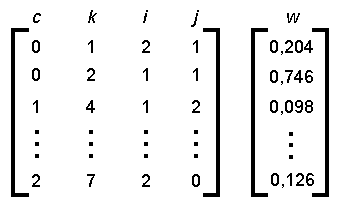
\includepdf[pages=-, width=6cm]{figuras/figx.pdf}
	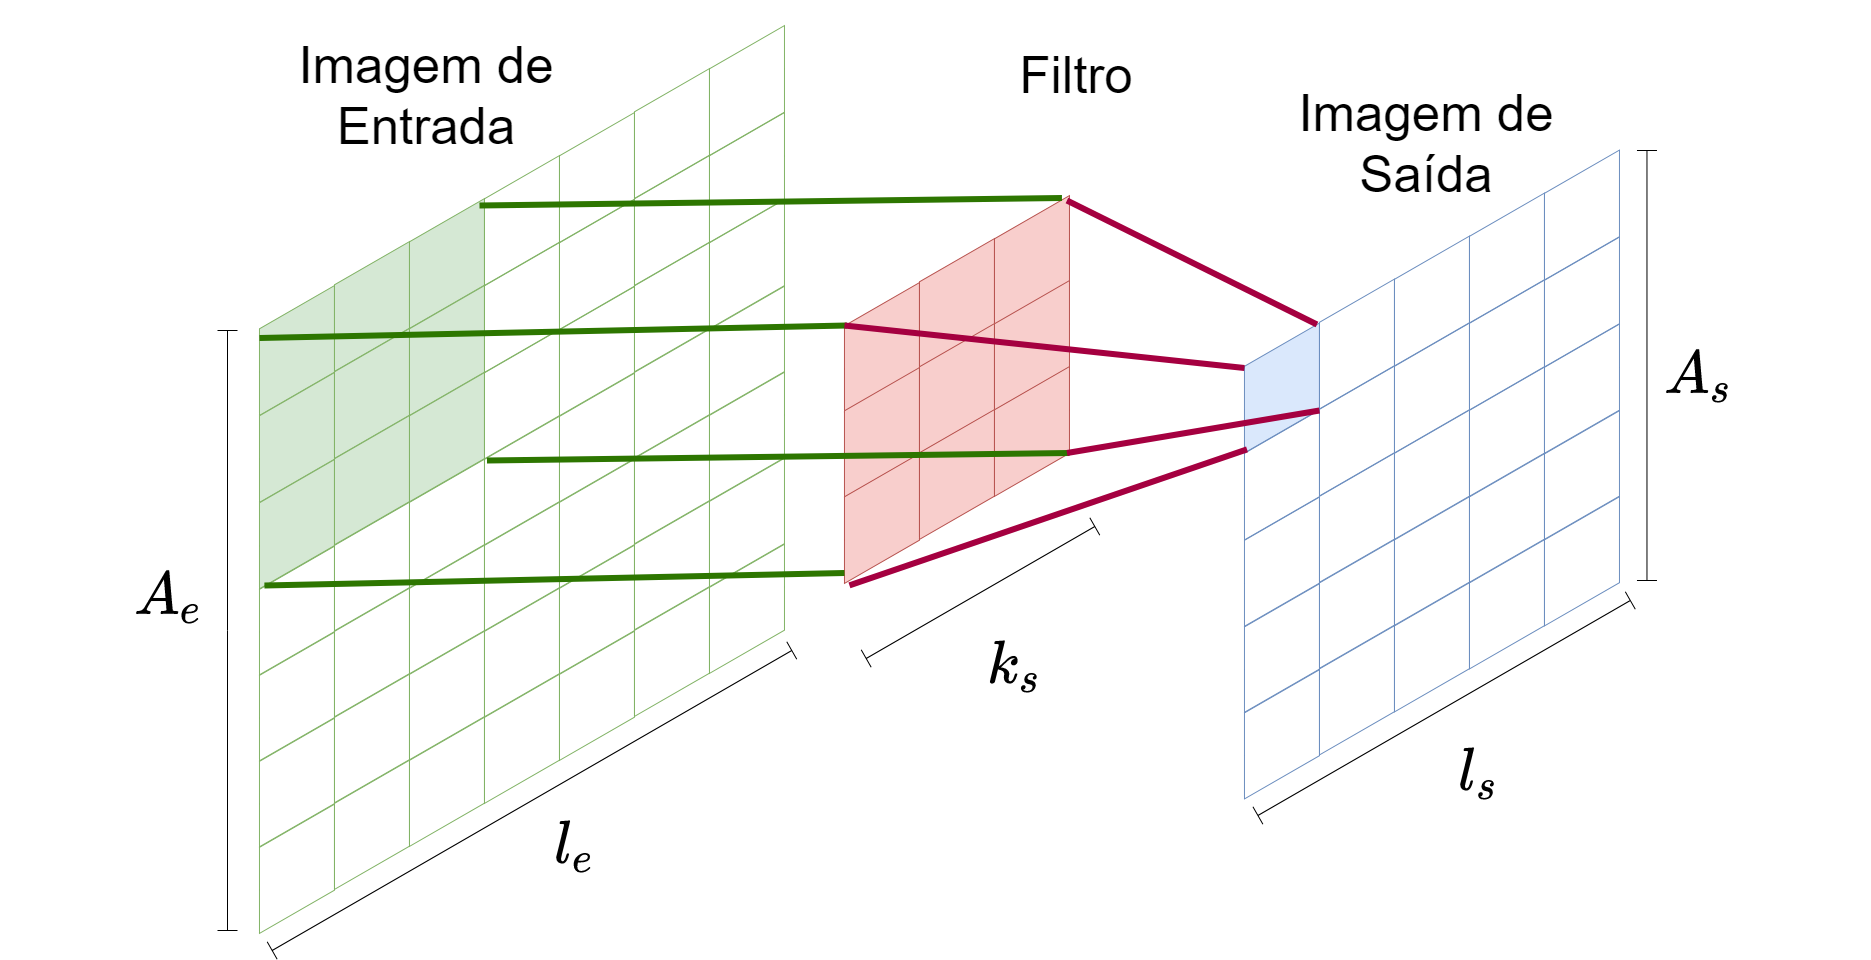
\includegraphics[width=0.45\textwidth, keepaspectratio=true]{figuras/CAP4/convv.png}
	\centering
	\caption[Operação de convolução]{Operação de convolução}
	\fonte{Elaborada pela autor.}
	%\label{fig:sharpe}
\end{figure}

\subsection{Camada de Agrupamento (\textit{Pooling})}
Na camada de agrupamento é realizado o processamento da imagem de entrada para redução da quantidade de parâmetros. Isso se faz selecionando, dentre um certo valor de parâmetros dentro da janela de \textit{pooling}, aquele que se adeque com o desejado. Normalmente, o agrupamento é feito a partir dos valores mais altos do grupo, através do \textit{max-polling}. Porém, o agrupamento pode ser realizado a partir do mínimo, do valor médio, entre outros.

Assim como a camada convolucional, é necessário escolher alguns hiperparâmetros para essa camada, como o tamanho da janela do agrupamento e o seu \textit{stride}. A Figura 2 apresenta a operação de \textit{max-pooling} para uma janela de agrupamento de tamanho 2 e \textit{stride} de 2, onde cada pixel da imagem de saída é o maior elemento dentro da janela de 4 elementos.

\begin{figure}[H]
    %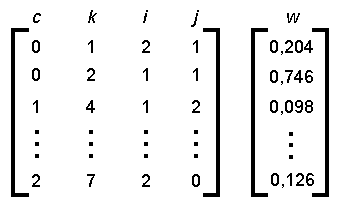
\includepdf[pages=-, width=6cm]{figuras/figx.pdf}
	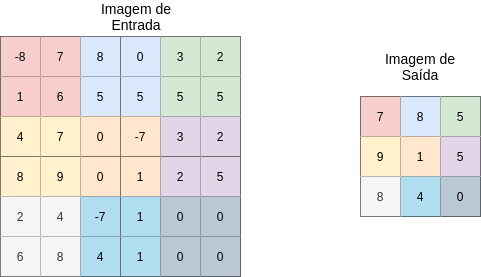
\includegraphics[width=0.5\textwidth, keepaspectratio=true]{figuras/poolig.png}
	\centering
	\caption[Operação de \textit{max-pooling}]{Operação de \textit{max-pooling}}
	\fonte{Elaborada pela autor.}
	%\label{fig:sharpe}
\end{figure}

\subsection{Camada de \textit{flattening}}

A Figura 3 ilustra o processo de flattening, que é responsável por realiza uma transformação na matriz da imagem, alterando seu formato para um vetor. Por exemplo, se a entrada da camada de \textit{flattening} for uma matriz de 32x32x3, a saída será um vetor de 3072 posições.

\begin{figure}[H]
    %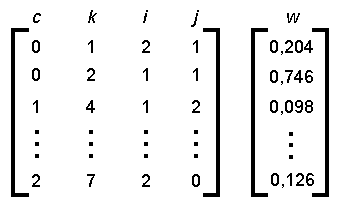
\includepdf[pages=-, width=6cm]{figuras/figx.pdf}
	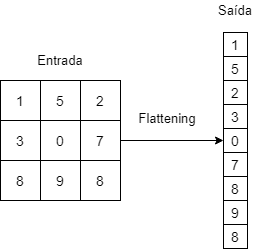
\includegraphics[width=0.22\textwidth, keepaspectratio=true]{figuras/flatten (1).png}
	\centering
	\caption[Operação de \textit{flattening}]{Operação de \textit{flattening}}
	\fonte{Elaborada pela autor.}
	%\label{fig:sharpe}
\end{figure}

\subsection{Camada \textit{fully-connected} (totalmente conectada)}
A camada totalmente conectada é a camada mais utilizada em aplicações de redes neurais. Ela se forma a partir da conexão de todos os neurônios de entrada e saída por pesos. Como hiperparâmetro, pode-se definir a quantidade de parâmetros a serem utilizados. A Figura 4 apresenta um modelo convencional de camadas totalmente conectadas.

\begin{figure}[H]
    %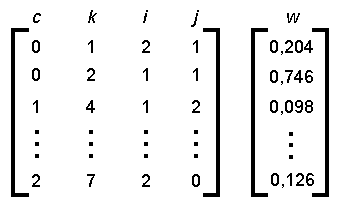
\includepdf[pages=-, width=6cm]{figuras/figx.pdf}
	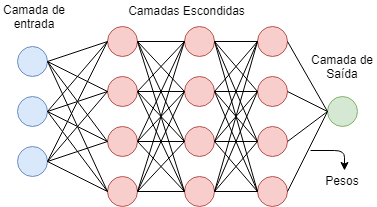
\includegraphics[width=0.35\textwidth, keepaspectratio=true]{figuras/rede.png}
	\centering
	\caption[Estrutura e operações da camada \textit{fully-connected}]{Estrutura e operações da camada \textit{fully-connected}}
	\fonte{Elaborada pela autor.}
	%\label{fig:sharpe}
\end{figure}

A Figura 5 ilustra as operações realizadas entre entre os neurônios e os pesos, onde $X_n$ é o valor armazenado no \textit{n}-ésimo neurônio e $w_n$ é o peso que conecta o neurônio da camada anterior com o neurônio da camada atual.

\begin{figure}[H]
    %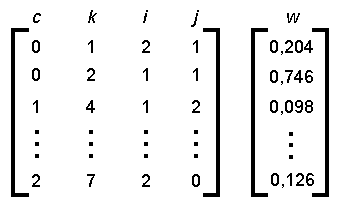
\includepdf[pages=-, width=6cm]{figuras/figx.pdf}
	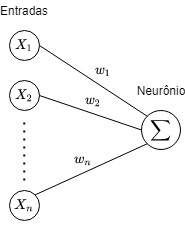
\includegraphics[width=0.2\textwidth, keepaspectratio=true]{figuras/rna.png}
	\centering
	\caption[Operações realizadas na camada \textit{fully-connected}]{Operações realizadas na camada \textit{fully-connected}}
	\fonte{Elaborada pela autor.}
	%\label{fig:sharpe}
\end{figure}

\subsection{Funções de ativação}
A aplicação da função de ativação pode ser utilizada em qualquer camada da rede. Ela é a transformação não linear que é feita ao longo da entrada. A saída desta função é enviada para a próxima camada. Uma rede neural sem função de ativação torna-se apenas um modelo linear, sendo que a maioria dos problemas complexos resolvidos por redes neurais são não-lineares.

Existem diversas funções de ativação diferentes. Para este trabalho foram utilizadas apenas duas: a ReLU e a softmax. A função ReLU é definida na Equação 2.3, onde $y$ é a saída da função que retorna o valor máximo entre 0 e o valor de $x$, que é o parâmetro sendo analisado. A Figura 6 mostra o gráfico dessa função.

\begin{equation}
    y = max(0,x)
\end{equation}

\begin{figure}[H]
    %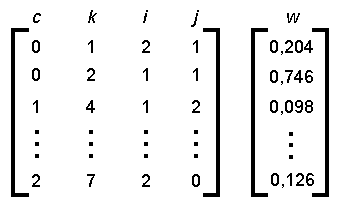
\includepdf[pages=-, width=6cm]{figuras/figx.pdf}
	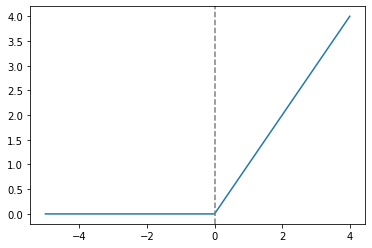
\includegraphics[width=0.4\textwidth, keepaspectratio=true]{figuras/relu.png}
	\centering
	\caption[Função de ativação ReLU]{Função de ativação ReLU}
	\fonte{Elaborada pela autor.}
	%\label{fig:sharpe}
\end{figure}

A função de ativação softmax, também conhecida como softargmax ou função exponencial normalizada, é uma função que recebe um vetor com \textit{z} números reais e o normaliza em uma distribuição probabilistica para os \textit{z} valores. Essa função é normalmente utilizada na camada de saída para que seja representada a probabilidade da imagem em análise pertencer a cada uma das classes. Essa função é definida na Equação 2.4, onde $z_i$ é o \textit{i}-ésimo termo do vetor z e $z_j$ é o \textit{j}-ésimo termo do mesmo vetor. Essa função é representada graficamente na Figura 7.

\begin{equation}
    S(z_i) = \frac{e^{z_i}}{\sum_{j=1}^k e^{z_j}}
\end{equation}

\begin{figure}[H]
    %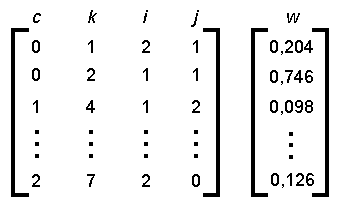
\includepdf[pages=-, width=6cm]{figuras/figx.pdf}
	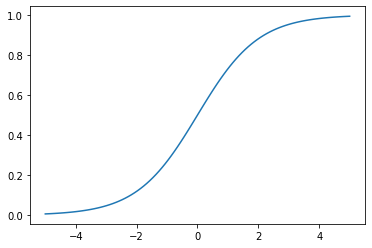
\includegraphics[width=0.4\textwidth, keepaspectratio=true]{figuras/softmax.png}
	\centering
	\caption[Função de ativação softmax]{Função de ativação softmax}
	\fonte{Elaborada pela autor.}
	%\label{fig:sharpe}
\end{figure}

\section{Técnicas de compressão de modelo} \label{secao1}
As estratégias para aceleração de inferência podem ser classificadas em baseadas em algoritmos e baseada em sistemas. Abordagens de aceleração baseadas em algorítmos incluem: processamento paralelo, compressão de modelo, exploração de esparsidade e redução de modelo por aproximação. Já as abordagens de aceleração baseadas em sistemas abrangem sistemas de memória de alta largura de banda para minimizar o tempo de acesso à memória, aceleradores de hardware, sistemas de computação distribuída e otimizações de compilador, como eliminação de expressão comum. A estratégia baseada em algoritmos usando compresão, foco deste trabalho, é uma forma comum na redução do número de operações nas redes neurais profundas.


\subsection{Exploração de esparsidade}

Uma matriz é dita esparsa quando a maior parte de seus elementos são zeros. A exploração da esparsidade pode estar presente em multiplos níveis: \textit{bit}, valor, canal, filtro, bloco entre outros. O valor da esparsidade de certa camada, ou modelo, é encontrado a partir da Equação 2.5, onde $n_{zeros}$ representa a quantidade de zeros e $n_{pesos}$ representa a quantidade de pesos.

\begin{equation}
    esparsidade = \frac{n_{zeros}}{n_{pesos}}*100%
\end{equation}

A esparsidade também pode ser computada a partir da contagem de elementos com magnitude muito próximas a zero, ou não significativos. A Tabela 1 apresenta um exemplo da esparsidade de uma rede neural com 65536 parâmetos, onde $W_k$ representa o limite que define a magnitude dos pesos que são considerados insignificantes para o modelo a coluna de Quantidade de pesos mostra quantos pesos são removidos para cada limite de $W_k$ e a teceira coluna mostra as esparsidades do modelo.

\begin{table}[H]
    \centering
    \begin{tabular}{ |p{3cm}|p{3cm}|p{3cm}|  }
 %\hline
 %\multicolumn{2}{|c|}{Estrutura da rede utilizada} \\
 \hline
 Mag. do peso&Qtd. de pesos&Esparsidade \\
 \hline
    $W_k$ < 0.01            &6438    &   9,82\%\\
    $W_k$ < 0.001           &3220    &   4,91\%\\
    $W_k$ < 0.0001          &1924    &   2,94\%\\
 \hline
 \multicolumn{3}{|c|}{Rede neural com 65536 pesos} \\
 \hline
\end{tabular}
    \caption{Esparsidade para pesos com diferentes magnitudes}
    \label{tab:my_label}
\end{table}

\subsection{Compressão de modelo por poda}
Atualmente, diferentes técnicas de compressão de modelo são utilizados, como quantização da rede, poda e ajuste fino de modelos pré-treinados. A compressão de modelo também pode ser realizada a partir da quantização seguida da poda ou da poda seguida da quantização. 

A otimização utilizando a técnica de poda, objeto deste trabalho, consiste na remoção de pesos insignificantes do modelo a partir de um certo \textit{threshold} (limiar). A definição deste limiar expressa o quão agressiva será a poda no modelo, sendo que a remoção de muitos pesos pode afeter significativamente a acurácia da rede. A remoção desses pesos faz com que a quantidade de operações realizadas durante a inferêmcia da rede seja menor que a do modelo não comprimido. A figura 8 mostra como acontece a remoção dos pesos do modelo.

\begin{figure}[H]
    %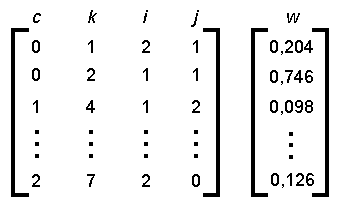
\includepdf[pages=-, width=6cm]{figuras/figx.pdf}
	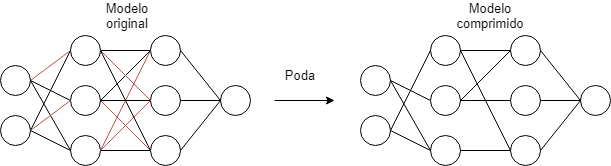
\includegraphics[width=0.6\textwidth, keepaspectratio=true]{figuras/poda.png}
	\centering
	\caption[Representação da técnica de poda]{Representação da técnica de poda}
	\fonte{Elaborada pela autor.}
	%\label{fig:sharpe}
\end{figure}

A remoção dos pesos ocorre durante o loop de aprendizagem do modelo. As técnicas mais convencionais realizam a remoção dos pesos apenas no primeiro \textit{batch} de cada época, outras realizam o mesmo processo apenas no final de cada época. O \textit{loop} de aprendizado de \textit{prune-aware} pode ser visualizado na Figura 9. Onde $Y(n)$ é a classe predita do modelo para a entrada $X_n$, $Yref(n)$ é a classe real da entrada, $E(n)$ é o erro obtido pela diferença entre a saída predita e a saída real, $G(n)$ é a aplicação do gradiente de decida levando em consideração tanto o erro quanto os pesos removidos. $W(n)$ é o \textit{n}-ésimo peso, $Z^{-1}$ é um atraso e $C(n)$ é o resulado do peso que sofreu a poda. Para o controle do momento que deverá haver a poda, existe uma chave de controle de época que fecha ou abre o caminho com a remoção do peso quando desejado.


\begin{figure}[!h]
    %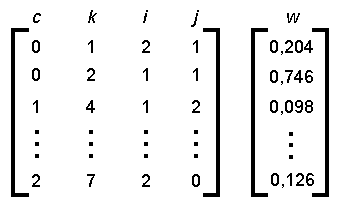
\includepdf[pages=-, width=6cm]{figuras/figx.pdf}
	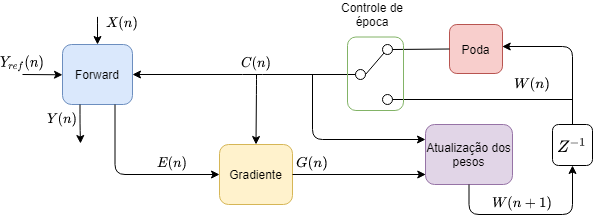
\includegraphics[width=0.7\textwidth, keepaspectratio=true]{figuras/prune_normal (1).png}
	\centering
	\caption[loop de aprendizado de \textit{prune-aware} convencional]{loop de aprendizado de \textit{prune-aware} convencional}
	\fonte{Elaborada pela autor.}
	%\label{fig:sharpe}
\end{figure}


%\section[\textit{Seção}]{\textit{Seção}}
%\lipsum[1-2]

%Itens em latex:
%\begin{itemize}
%	\item texto 1;
%	\item texto 2;
%	\item texto 3;
%\end{itemize}

%\lipsum[2-3]

%\subsection{Subseção}

%\lipsum[2-4]

% Capitulo 3
\chapter[Metodologia]{METODOLOGIA}
\label{ch:cap3}

Nesta seção, será apresentada de forma técnica e descritiva a metodologia utilizada para o desenvolvimento da ténica de compressão de redes neurais profundas por poda, análise dos resultados obtidos de acurácia e esparsidade para modelos sem utilização de poda e para podas mais agressivas.

A metodologia adotada para realizar os primeiros experimentos foi, inicialmente, a seleção dos dados a serem utilizados para classificação, definição do modelo de rede e definição das bibliotecas e o ambiente de desenvolvimento a ser utilizado. Após isso, foram definido os hiperparametrose as métricas a serem analisadas para os resultados obtidos. E então, o processo de aprendizagem foi realizado.

%O processo de aprendizagem foi realizado com os mesmos parâmetros sete vezes, sendo modificado apenas o valor de $ \alpha $, que define o quão agressiva é a poda. Além disso, também é computada a quantidade de pesos que foram removidos para o cáculo da esparsidade do modelo.

%Por fim, foram análisados os resultados obtidos, levando em consideração a quantidade de pesos significativos através da esparsidade final do modelo e a acurácia obtida. Com esses resultados, é possível montado a rede neural no hardware com a mesma estrutura e pesos do modelo treinado, removendo os pesos insignificantes.


%\begin{itemize}
%    \item Primeiro
%    \subitem - $C_1 > F_1 + F_2 $
%    \item Segundo
%    \subitem - $C_2 > F_1 + F_2 - C_1$
%\end{itemize}

%\begin{equation} \label{eq1}
%R(t) = P(T > t) = 1 - F(t)
%\end{equation}

\section{Proposta} \label{secao1}

Uma das características das redes neurais é a grande quantidade de operações numéricas realizadas durante os processos de treinamento e inferência. Nos hardwares, em geral, muitas operações matemáticas aumentam significativamente o seu consumo energético. Como resultado, aparelhos alimentados por bateria ainda não conseguem executar redes neurais convolucionais de ultima geração devido o seu limite energético \cite{yang2017}.

As técnicas de compressão mais convencionais realizam a poda somente no primeiro batch de cada época, ou ao final de cada época. A proposta é a realização da poda em todos os batches. A aplicação desta técnica já foi utilizada para classificação viral \cite{fernandes2021}, a proposta é utilizar a mesma ténica para classificação de imagens.


\subsection{Treinamento} \label{secao11}

A estratégia escolhida para redução da quantidade de operações númericas foi a de compressão por poda. Assim, durante o treinamento, foi aplicada a poda em todas as camadas do modelo baseados em um limiar ($ \beta_k $) definido pelo desvio padrão dos seus pesos multiplicados por uma constante $ \alpha_k $ determinada antes do processo de treinamento. Esta variável é que indica o quão agressiva será a compressão do modelo. Todos os pesos com magnitude menor que esse valor são removidos. 

O processo de aprendizado e compressão por poda pode ser vizualizado na Figura 10. Onde $Y(n)$ é a classe predita pelo modelo para a entrada $X(n)$. O erro $E(n)$ é calculado a partir da diferença entre a saída predita e $Y_{ref}(n)$ que é a classe real do dado de entrada. A partir do erro, é claculado o gradiente de descida $G(n)$ e então os pesos são atualizados. $C(n)$ são os pesos do modelo após o processo da poda. Os pesos que foram zerados também passam pelo cálculo do gradiente.

\begin{equation}
    \beta_k = \alpha * \sigma_k
\end{equation}

\begin{equation}
    C_k(n) = P(W_k(n),\beta_k) =
    \begin{cases}
      w_k(n) & \text{if } |w_k(n)|\geq \beta_k \\
      0 & \text{if } |w_k(n)| < \beta_k\\
    \end{cases} 
\end{equation}

A Equação 3.1 mostra como é feito o cálculo do limiar, sendo $ \beta_k $ o limiar da \textit{k}-ésima camada, $\alpha$ a constante que estabelece a agressividade da poda e $\sigma_k$ o desvio padrão da \textit{k}-ésima camada.

Na Equação 3.2 temos P(.,.), que representa a função de poda, é feita a análise se o \textit{n}-ésimo peso da \textit{k}-ésima camada é menor que o limiar calculado. Se for, o valor do peso passa a ser zero. As Figuras 12 e 13 apresentam um exemplo da remoção dos pesos para $ \alpha $ = 0.75, removendo um total de 15638 parâmetros dessa camada.

\begin{figure}[!h]
    %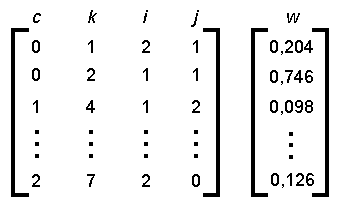
\includepdf[pages=-, width=6cm]{figuras/figx.pdf}
	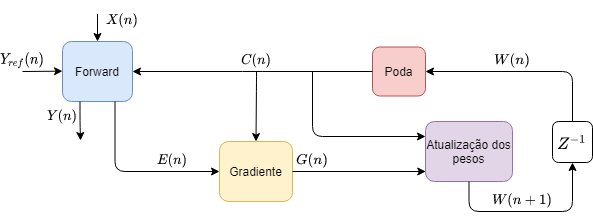
\includegraphics[width=0.7\textwidth, keepaspectratio=true]{figuras/diagram.png}
	\centering
	\caption[Diagrama de loop de aprendizado do \textit{pruning-aware}]{Diagrama de loop de aprendizado do \textit{pruning-aware}}
	\fonte{Elaborada pela autor.}
	%\label{fig:sharpe}
\end{figure}

A cada iteração do loop de aprendizado, foi contabilizada a quantidade de pesos que são removidos e, após isso, foi calculada a esparsidade do modelo, ou seja, a porcentagem de pesos insignificantes da rede. A análise da eficácia da poda é medida a partir da diferença entre as acurácias de de inferência entre o modelo sem compressão e o modelo com compressão.

\begin{figure}[H]
    %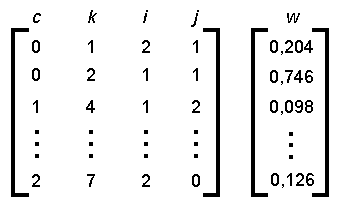
\includepdf[pages=-, width=6cm]{figuras/figx.pdf}
	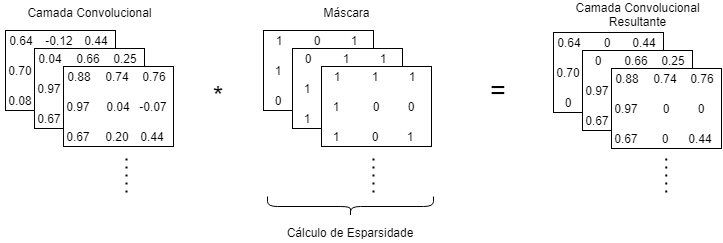
\includegraphics[width=0.8\textwidth, keepaspectratio=true]{figuras/tfmul.png}
	\centering
	\caption[Processo de remoção de pesos na camada convolucional]{Processo de remoção de pesos na camada convolucional}
	\fonte{Elaborada pela autor.}
	%\label{fig:sharpe}
\end{figure}

A remoção dos pesos foi realizada a partir da criação de uma máscara, com o mesmo formato da camada do modelo em análise. Cada índice da máscara é preenchido com zero ou um a depender da magnitude do peso associado na camada. Caso seu peso seja menor que o limiar definido, seu índice será zero, caso contrário será 1. A partir da multiplicação entre a camada e a máscara, é obtido como resultado a camada com os pesos a serem removidos e o valor da esparsidade a partir da contagem de pesos zerados. A figura 10 ilustra como funciona o processo de remoção de pesos. As Figuras 12 e 13 mostram o resultado da remoção dos pesos na segunda camada convolucional do modelo. Como pode ser visto na Tabela 2, a segunda camada convolucional possui 18.496 parâmetros, portanto, nesse exemplo, apenas 2.858 parâmetros possuem pesos significativos.




\begin{figure}[H]
    %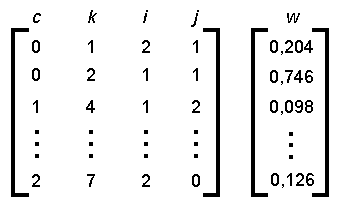
\includepdf[pages=-, width=6cm]{figuras/figx.pdf}
	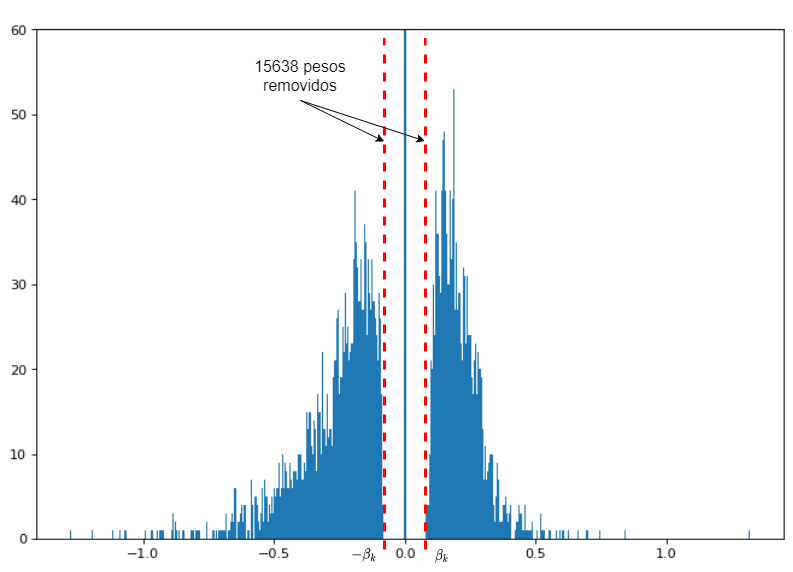
\includegraphics[width=0.65\textwidth, keepaspectratio=true]{figuras/antes (1).png}
	\centering
	\caption[Histograma de pesos da segunda camada convolucional antes da poda]{Histograma de pesos da segunda camada convolucional antes da poda}
	\fonte{Elaborada pela autor.}
	%\label{fig:sharpe}
\end{figure}

\begin{figure}[H]
    %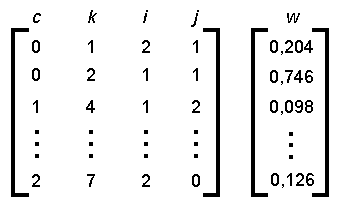
\includepdf[pages=-, width=6cm]{figuras/figx.pdf}
	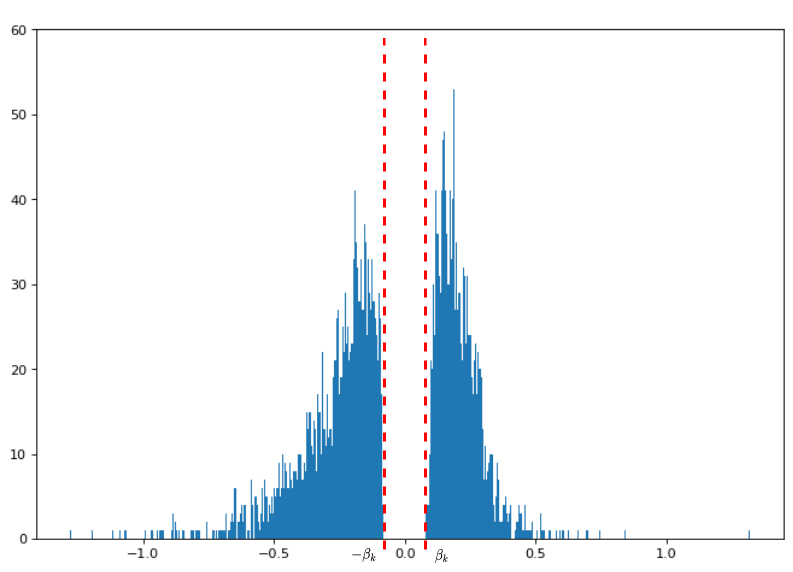
\includegraphics[width=0.65\textwidth, keepaspectratio=true]{figuras/depois.png}
	\centering
	\caption[Histograma de pesos da segunda camada convolucional depois da poda]{Histograma de pesos da segunda camada convolucional depois da poda}
	\fonte{Elaborada pela autor.}
	%\label{fig:sharpe}
\end{figure}

\subsection{Modelo e hiper-parâmetros} \label{secao12}
O processo de treinamento foi realizado sete vezes, variando em $\alpha$ = 0,00, $\alpha$ = 0,25, $\alpha$ = 0,50, $\alpha$ = 0,75, $\alpha$ = 1,00, $\alpha$ = 1,25 e $\alpha$ = 1,50. A função utilizada para cáculo das perdas foi a Sparse Categorical Corossentropy e a função do otimizador utilizada foi Adam. Em todos os experimentos, a estrutura da rede foi criada da seguinte forma:

\begin{enumerate}
   \item Camada de entrada de 32x32x3;
   \item Camada convolucional com 32 kernels de 3x3, sem padding, stride igual a 1 e função de ativição relu;
   \item Camada convolucional com 64 kernels de 3x3, sem padding, stride igual a 1 e função de ativição relu;
   \item Camada de Max-pooling de 2x2, stride igual a 2;
   \item Camada convolucional com 128 kernels de 3x3, sem padding, stride igual a 1 e função de ativição relu;
   \item Camada convolucional com 128 kernels de 3x3, sem padding, stride igual a 1 e função de ativição relu;
   \item Camada de Max-pooling de 2x2, stride igual a 2;
   \item Camada totalmente conectada com 256 neurônios e função de ativação relu;
   \item Camada totalmente conectada com 128 neurônios e função de ativação relu;
   \item Camada de saída para 10 classes com função de ativação softmax.
\end{enumerate}

A tabela 2 mostra a quantidade de parâmetros de cada camada e também de todo o modelo.

\begin{table}[H]
    \centering
    \begin{tabular}{ |p{4cm}|p{3cm}|  }
 %\hline
 %\multicolumn{2}{|c|}{Estrutura da rede utilizada} \\
 \hline
 Tipo de Camada&Quantidade de parâmetros \\
 \hline
    Convolucional 2D        &896    \\
    Convolucional 2D        &18.496    \\
    Max Pooling 2D          &0    \\
    Convolucional 2D        &73.856    \\
    Convolucional 2D        &147.584    \\
    Max Pooling 2D          &0    \\
    Flatten                 &0    \\
    Dense                   &819.456    \\
    Dense                   &32.896    \\
    Dense                   &1.290    \\
    
 \hline
 \multicolumn{2}{|c|}{Total de 1.094.474 parâmetros} \\
 \hline
\end{tabular}
    \caption{Quantidade de parâmetros da rede}
    \label{tab:my_label}
\end{table}












%\subsection{Análise em hardware} \label{section13}

%Após o processo de aprendizagem com compressão, o modelo resultante foi desenvolvido em um hardware de baixo consumo. Para isso, foram feitas algumas modificações no formato do modelo. Foi criado uma matriz armazenando apenas os índices e pesos significativos de cada camada e um vetor contendo o valor dos pesos de forma que uma linha da matriz represente os índices do peso da mesma linha do vetor de pesos. A figura 5 apresenta um exemplo para uma camada convolucional, com \textit{c} representando o canal, \textit{k} representando o \textit{kernel} (filtro), \textit{i} e \textit{j} representando o linha e coluna do peso no kernel e \textit{w} como peso.



%\subsection{Validação} \label{section14}
%Para validar se realmente houve uma diminuição da necessidade do esforço computacional no hardware, primeiro, foi contabilizado a quantidade de pulsos de clock necessários para uma simples operação matemática de multiplicação e soma. Em seguida, foi contabilizado a quantidade de operações numéricas que devem ser realizadas pelo microcontrolador em todo o modelo de acordo com sua esparsidade. Após isso, foi verificado a quantidade de pulsos de clock necessários para que uma certa amostra passe por todo modelo. Por fim, foi verificado se a quantidade de pulsos de clock para operações em todo o modelo estava de acordo com a prevista pela multiplicação entre a quantidade de clocks para uma única operação e a quantidade de operações a serem realizadas no modelo.

%Use \textit{labels} para criar links para as seções, como \autoref{secao1}.

%\lipsum[5-8]


\section{Dataset} \label{secao2}

O dataset escolhido para esse trabalho chama-se CIFAR-10, que consiste em 60 mil imagens coloridas com 3 canais (RGB) de 32x32 pixels divididas em 10 classes, com 6 mil imagens de cada classe. O dataset é dividido em 50 mil imagens para treino e 10 mil para inferência. 

\begin{figure}[H]
    %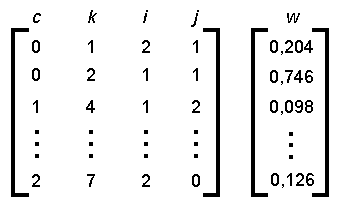
\includepdf[pages=-, width=6cm]{figuras/figx.pdf}
	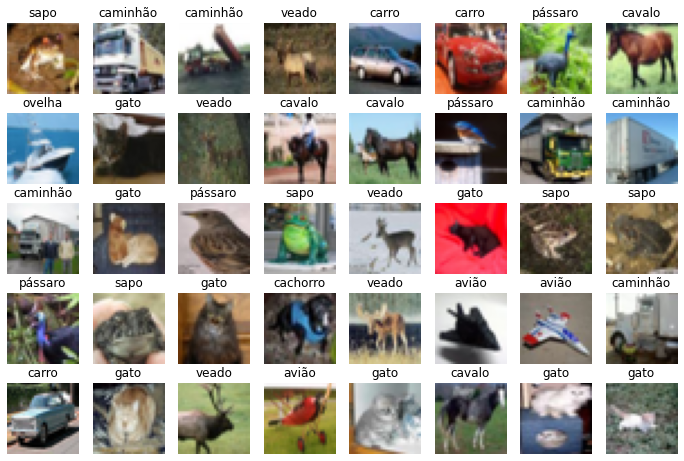
\includegraphics[width=0.7\textwidth, keepaspectratio=true]{figuras/cifar10ex.png}
	\centering
	\caption[Amostras do dataset CIFAR-10]{Amostras do dataset CIFAR-10}
	\fonte{Elaborada pela autor.}
	%\label{fig:sharpe}
\end{figure}




As 10 classes são: avião, automóvel, pássaro, gato, veado, cachorro, sapo, cavalo, barco e caminhão. As classes são exclusivas entre si, ou seja, não há sobreposição entre automóveis e caminhões. A classe de automóveis inclui apenas sedans, SUV's e carros de pequeno porte. A classe de caminhão inclue apenas caminhões grandes, excluindo pickups. A Figura 14 apresenta algumas amostras do dataset.

% Capitulo 4
\chapter[Resultados]{Resultados}
\label{ch:cap4}
%\lipsum[3-5]

Neste capitulo serão apresentados os resultados obtidos e serão feitas algumas observações a respeito desses resultados a partir da modificação do limiar $\alpha$ em sete valores diferentes. Primeiramente, serão apresentados os dados obtidos para cada limiar e após isso será feita a comparação entre os resultados.

\section{Resultados obtidos para diferentes valores do Limiar}
Os resultados apresentados nesta seção foram obtidos a partir da modificação do limiar antes do processo de aprendizagem. Essa modificação é realizada a partir da alteração da consetante $\alpha$ como ja apresentado nos capítulos anteriores deste trabalho.


\subsection{$\alpha$ = 0}
O primeiro experimento realizado foi utilizando o $\alpha$ = 0, ou seja, não é realizada nenhuma poda no modelo. O primeiro experimento foi executado sem poda para futuras comparações entre o modelo otimizado e o não otimizado. Dessa forma, a esparsidade final é igual a 0\%. A partir da Figura 15, é possível ver a variação dos valores de acurácia de treinamento e de validação durante as 30 épocas.

\begin{figure}[H]
    %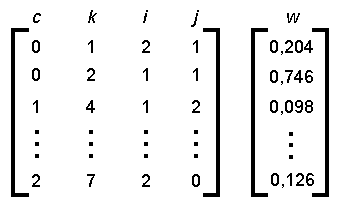
\includepdf[pages=-, width=6cm]{figuras/figx.pdf}
	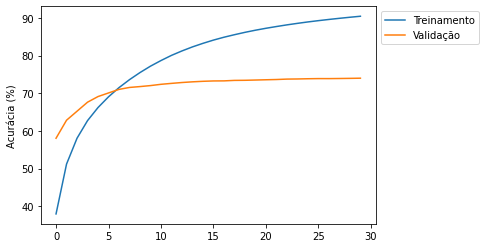
\includegraphics[width=0.6\textwidth, keepaspectratio=true]{figuras/CAP4/acuracia0.png}
	\centering
	\caption[Acurácia de treinamento e validação para $\alpha$ = 0]{Acurácia de treinamento e validação para $\alpha$ = 0}
	\fonte{Elaborada pela autor.}
	%\label{fig:sharpe}
\end{figure}

Para analisar o comportamento dos pesos ao final do treinamento, foi montado um histograma contendo todos os pesos da segunda camada convolucional do modelo, como visto na Figura 16. É possível perceber que uma grande quantidade de pesos se concentram em valores próximos a zero.

\begin{figure}[H]
    %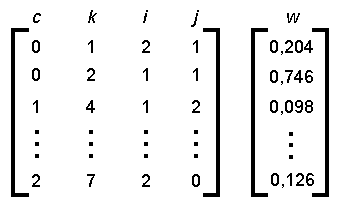
\includepdf[pages=-, width=6cm]{figuras/figx.pdf}
	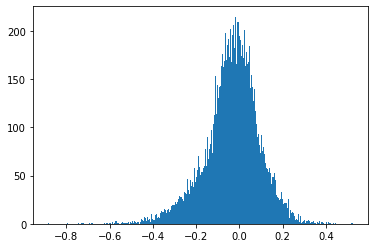
\includegraphics[width=0.5\textwidth, keepaspectratio=true]{figuras/CAP4/hist0_.png}
	\centering
	\caption[Histograma de pesos da segunda camada convolucional do modelo para $\alpha$ = 0]{Histograma de pesos da segunda camada convolucional do modelo para $\alpha$ = 0}
	\fonte{Elaborada pela autor.}
	%\label{fig:sharpe}
\end{figure}

No processo de inferência, obteve-se uma acurácia de 75,30\%. Para visualização dos resultados, a Figura 17 mostra a matriz de confusão obtida. 

\begin{figure}[H]
    %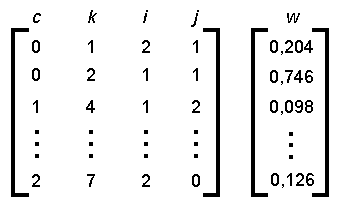
\includepdf[pages=-, width=6cm]{figuras/figx.pdf}
	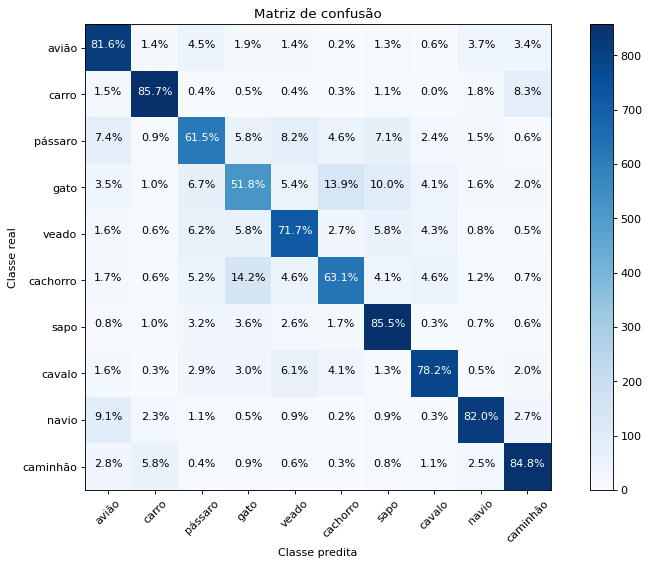
\includegraphics[width=0.7\textwidth, keepaspectratio=true]{figuras/CAP4/cm_0_.png}
	\centering
	\caption[Matriz de confusão para $\alpha$ = 0]{Matriz de confusão para $\alpha$ = 0}
	\fonte{Elaborada pela autor.}
	%\label{fig:sharpe}
\end{figure}


\subsection{$\alpha$ = 0,25}
Após o experimento realizado sem compressão, foi realizado o mesmo processo de treinamento, porém o $\alpha$ foi alterado para 0,25, sendo esse o valor menos agressivo de poda realizado durante todos os experimentos. Dessa vez, o modelo apresentará esparsidade maior que 0\%, uma vez que haverá poda. A Figura 18 mostra a acurácia de e treinamento e validação para o novo valor do limiar. Já a variação da esparsidade durante as épocas pode ser vizualizada na Figura 19. A esparsidade final do modelo chegou a 52,72\%.

\begin{figure}[H]
    %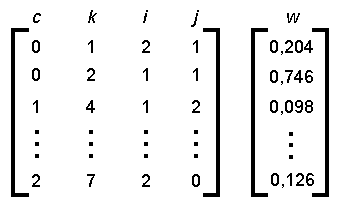
\includepdf[pages=-, width=6cm]{figuras/figx.pdf}
	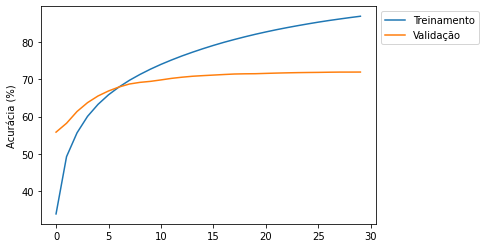
\includegraphics[width=0.6\textwidth, keepaspectratio=true]{figuras/CAP4/acuracia025.png}
	\centering
	\caption[Acurácia de treinamento e validação para $\alpha$ = 0,25]{Acurácia de treinamento e validação para $\alpha$ = 0,25}
	\fonte{Elaborada pela autor.}
	%\label{fig:sharpe}
\end{figure}

\begin{figure}[H]
    %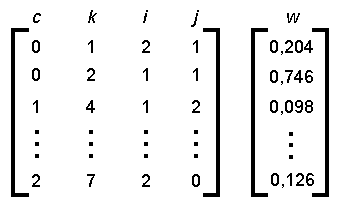
\includepdf[pages=-, width=6cm]{figuras/figx.pdf}
	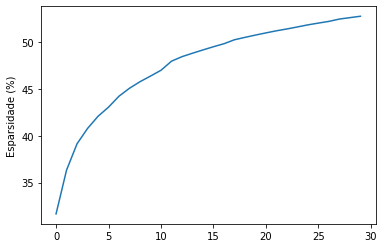
\includegraphics[width=0.5\textwidth, keepaspectratio=true]{figuras/CAP4/esparsidade025.png}
	\centering
	\caption[Variação da esparsidade durante as épocas para $\alpha$ = 0,25]{Variação da esparsidade durante as épocas para $\alpha$ = 0,25}
	\fonte{Elaborada pela autor.}
	%\label{fig:sharpe}
\end{figure}

A Figura 20 contém o histograma dos pesos da segunda camada convolucional. Devido o processo de compressão há uma grande concentração de pesos com valores muito próximos de zero, ou seja, os pesos a serem removidos por não terem grande influência no processo de classificação. Por esse motivo, foi necessário ampliar o histograma para verificar os pesos maiores que o limiar, como apresentado na Figura 21. 


\begin{figure}[H]
	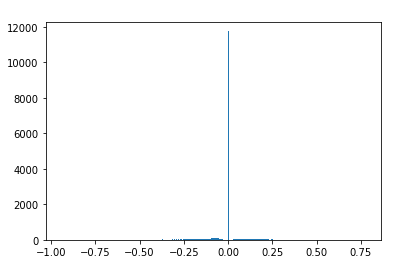
\includegraphics[width=0.5\textwidth, keepaspectratio=true]{figuras/CAP4/hist1_025_.png}
	\centering
	\caption[Histograma de pesos da segunda camada convolucional para $\alpha$ = 0,25]{Histograma de pesos da segunda camada convolucional para $\alpha$ = 0,25}
	\fonte{Elaborada pela autor.}
	%\label{fig:sharpe}
\end{figure}

\begin{figure}[H]
    %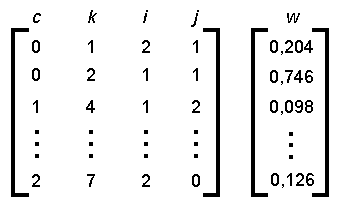
\includepdf[pages=-, width=6cm]{figuras/figx.pdf}
	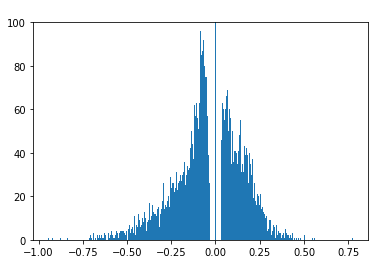
\includegraphics[width=0.5\textwidth, keepaspectratio=true]{figuras/CAP4/hist2_025_.png}
	\centering
	\caption[Histograma ampliado de pesos da segunda camada convolucional para $\alpha$ = 0,25]{Histograma de pesos da segunda camada convolucional para $\alpha$ = 0,25}
	\fonte{Elaborada pela autor.}
	%\label{fig:sharpe}
\end{figure}

No processo de inferência, foi obtida uma acurácia de 73,25\%, ou seja, quando comparado ao modelo não comprimido, é possível remover 52,72\% dos pesos e obter uma acurácia apenas 2,05\% menor. É possível analisar o resultado a partir da matriz de confusão na Figura  22.


\begin{figure}[H]
    %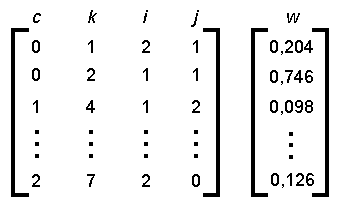
\includepdf[pages=-, width=6cm]{figuras/figx.pdf}
	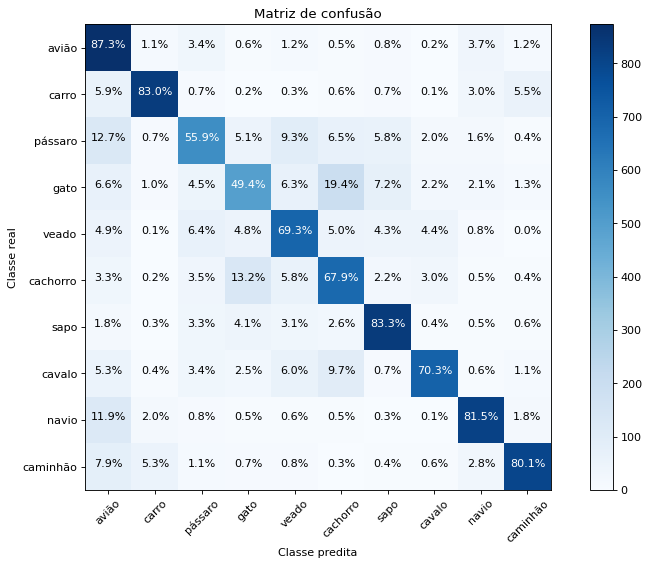
\includegraphics[width=0.68\textwidth, keepaspectratio=true]{figuras/CAP4/cm_025_.png}
	\centering
	\caption[Matriz de confusão para $\alpha$ = 0,25]{Matriz de confusão para $\alpha$ = 0,25}
	\fonte{Elaborada pela autor.}
	%\label{fig:sharpe}
\end{figure}


\subsection{$\alpha$ = 0,50}
O terceiro experimento consistiu em manter o mesmo processo de treinamento e inferência, mas dessa vez alterando o valor de $\alpha$ para 0,50. A Figura 23 apresenta o valor das acurácias de treino e validação para o modelo nessas configurações e a Figura 24 mostra a variação da esparsidade.A esparsidade do modelo chegou a aproximadamente 68,25\%.






\begin{figure}[H]
    %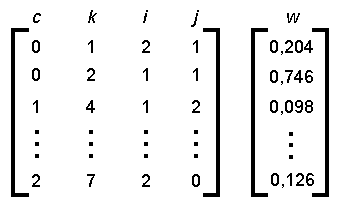
\includepdf[pages=-, width=6cm]{figuras/figx.pdf}
	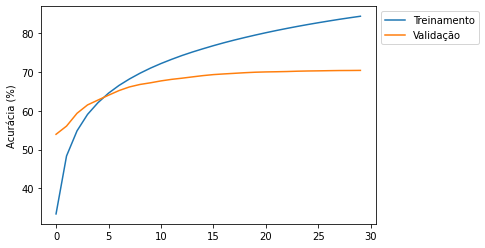
\includegraphics[width=0.6\textwidth, keepaspectratio=true]{figuras/CAP4/acuracia05.png}
	\centering
	\caption[Acurácia de treinamento e validação para $\alpha$ = 0,50]{Acurácia de treinamento e validação para $\alpha$ = 0,50}
	\fonte{Elaborada pela autor.}
	%\label{fig:sharpe}
\end{figure}

Assim como no experimento anterior, foi visualizado o histograma de pesos da segunda camada convolucional. Como a quantidade de pesos próximos a zero foi muito alta, foi impossível analisar os pesos com valores mais altos, em módulo, que o limiar. Portanto, a Figura 25 apresenta o histograma de pesos já ampliado.

Com o fim do treinamento, foi feita a inferência no modelo. O resultado foi uma acurácia de 71,90\%, mostrando que é possível remover aproximadamente 68,25\% dos parâmetros do modelo e obter uma acurácia apenas 3,4\% menor que a do modelo não comprimido. A matriz de confusão pode ser visualizada na Figura 26.

\begin{figure}[H]
    %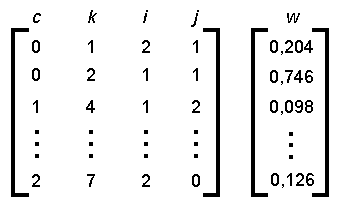
\includepdf[pages=-, width=6cm]{figuras/figx.pdf}
	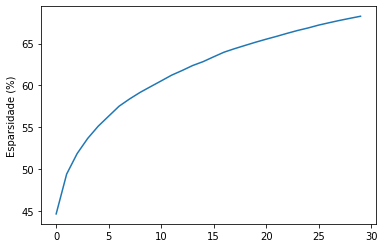
\includegraphics[width=0.5\textwidth, keepaspectratio=true]{figuras/CAP4/esparsidade05.png}
	\centering
	\caption[Variação da esparsidade durante as épocas para $\alpha$ = 0,50]{Variação da esparsidade durante as épocas para $\alpha$ = 0,50}
	\fonte{Elaborada pela autor.}
	%\label{fig:sharpe}
\end{figure}

\begin{figure}[H]
    %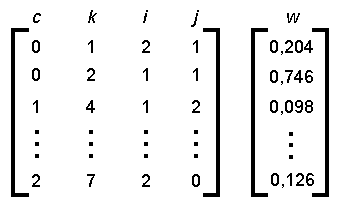
\includepdf[pages=-, width=6cm]{figuras/figx.pdf}
	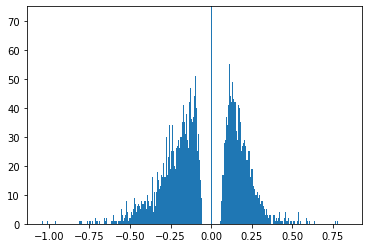
\includegraphics[width=0.5\textwidth, keepaspectratio=true]{figuras/CAP4/hist_50_.png}
	\centering
	\caption[Histograma de pesos da segunda camada convolucional para $\alpha$ = 0,50]{Histograma de pesos da segunda camada convolucional para $\alpha$ = 0,50}
	\fonte{Elaborada pela autor.}
	%\label{fig:sharpe}
\end{figure}

\begin{figure}[H]
    %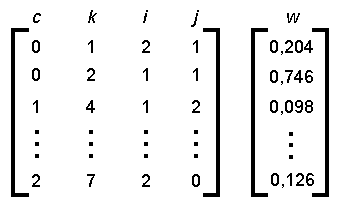
\includepdf[pages=-, width=6cm]{figuras/figx.pdf}
	\includegraphics[width=0.65\textwidth, keepaspectratio=true]{figuras/CAP4/cm_05_.png}
	\centering
	\caption[Matriz de confusão para $\alpha$ = 0,50]{Matriz de confusão para $\alpha$ = 0,50}
	\fonte{Elaborada pela autor.}
	%\label{fig:sharpe}
\end{figure}



\subsection{$\alpha$ = 0,75}

Os próximos resultados são obtidos a partir do mesmo procedimento dos experimentos anteriores, porém com $\alpha$ = 0,75. As acurácias de treinamento e validação podem ser observadas na Figura 27 e a variação da esparsidade durante o treinamento pode ser visualizada na Figura 28. A esparsidade final do modelo foi de 82,30\%. O histograma de pesos pode ser visto na Figura 29.


\begin{figure}[H]
    %\includepdf[pages=-, width=6cm]{figuras/figx.pdf}
	\includegraphics[width=0.6\textwidth, keepaspectratio=true]{figuras/CAP4/acuracia075.png}
	\centering
	\caption[Acurácia de treinamento e validação para $\alpha$ = 0,75]{Acurácia de treinamento e validação para $\alpha$ = 0,75}
	\fonte{Elaborada pela autor.}
	%\label{fig:sharpe}
\end{figure}

\begin{figure}[H]
    %\includepdf[pages=-, width=6cm]{figuras/figx.pdf}
	\includegraphics[width=0.5\textwidth, keepaspectratio=true]{figuras/CAP4/esparsidade075.png}
	\centering
	\caption[Variação da esparsidade durante as épocas para $\alpha$ = 0,75]{Variação da esparsidade durante as épocas para $\alpha$ = 0,75}
	\fonte{Elaborada pela autor.}
	%\label{fig:sharpe}
\end{figure}

\begin{figure}[H]
    %\includepdf[pages=-, width=6cm]{figuras/figx.pdf}
	\includegraphics[width=0.5\textwidth, keepaspectratio=true]{figuras/CAP4/hist075_.png}
	\centering
	\caption[Histograma de pesos da segunda camada convolucional para $\alpha$ = 0,75]{Histograma de pesos da segunda camada convolucional para $\alpha$ = 0,75}
	\fonte{Elaborada pela autor.}
	%\label{fig:sharpe}
\end{figure}

Dessa vez, a acurácia de inferência foi de 71,84\%, sendo possível então a remoção de 82,30\% dos parâmetros do modelo para obteção de uma acurácia de inferência apenas 3,46\% menor que a da rede neural não comprimida. A matriz de confusão pode ser visualizada na Figura 30.

\begin{figure}[H]
    %\includepdf[pages=-, width=6cm]{figuras/figx.pdf}
	\includegraphics[width=0.65\textwidth, keepaspectratio=true]{figuras/CAP4/cm075_.png}
	\centering
	\caption[Matriz de confusão para $\alpha$ = 0,75]{Matriz de confusão para $\alpha$ = 0,75}
	\fonte{Elaborada pela autor.}
	%\label{fig:sharpe}
\end{figure}




\subsection{$\alpha$ = 1,00}
O próximo experimento foi realizado com o $\alpha$ igual a 1,00. Desta vez o limiar será igual ao desvio padrão da camada. É possível vizualizar as acurácias de treinamento e validação na Figura 31 e a variação da esparsidade na Figura 32. Ao final do processo de aprendizagem, a esparsidade foi de 92,44\%.

\begin{figure}[H]
    %\includepdf[pages=-, width=6cm]{figuras/figx.pdf}
	\includegraphics[width=0.6\textwidth, keepaspectratio=true]{figuras/CAP4/acuracia10.png}
	\centering
	\caption[Acurácia de treinamento e validação para $\alpha$ = 1,00]{Acurácia de treinamento e validação para $\alpha$ = 1,00}
	\fonte{Elaborada pela autor.}
	%\label{fig:sharpe}
\end{figure}

A Figura 33 aprensenta o histograma de pesos após o processo de compressão por poda da segunda camada convolucional. A Figura 34 mostra a matriz de confusão da inferência do modelo.

Para este experimento, a acurácia de inferência obtida foi de 67,13\%, sendo então possível obter uma acurácia 7,17\% menor que a do modelo não comprimido ao se remover 92,44\% dos seus parâmetros.

\begin{figure}[H]
    %\includepdf[pages=-, width=6cm]{figuras/figx.pdf}
	\includegraphics[width=0.5\textwidth, keepaspectratio=true]{figuras/CAP4/esparsidade10.png}
	\centering
	\caption[Variação da esparsidade durante as épocas para $\alpha$ = 1,00]{Variação da esparsidade durante as épocas para $\alpha$ = 1,00}
	\fonte{Elaborada pela autor.}
	%\label{fig:sharpe}
\end{figure}

\begin{figure}[H]
    %\includepdf[pages=-, width=6cm]{figuras/figx.pdf}
	\includegraphics[width=0.5\textwidth, keepaspectratio=true]{figuras/CAP4/hist10_.png}
	\centering
	\caption[Histograma de pesos da segunda camada convolucional para $\alpha$ = 1,00]{Histograma de pesos da segunda camada convolucional para $\alpha$ = 1,00}
	\fonte{Elaborada pela autor.}
	%\label{fig:sharpe}
\end{figure}

\begin{figure}[H]
    %\includepdf[pages=-, width=6cm]{figuras/figx.pdf}
	\includegraphics[width=0.65\textwidth, keepaspectratio=true]{figuras/CAP4/cm10_.png}
	\centering
	\caption[Matriz de confusão para $\alpha$ = 1,00]{Matriz de confusão para $\alpha$ = 1,00}
	\fonte{Elaborada pela autor.}
	%\label{fig:sharpe}
\end{figure}


\subsection{$\alpha$ = 1,25}
Neste experimento, o valor de $\alpha$ foi modificado para 1,25 resultando em uma maior agressividade na remoção dos pesos. As acurácias de treinamento e validação podem ser visualizadas na Figura 35, enquanto o comportamento da esparsidade no decorrer do treinamento pode ser visto na Figura 36. A esparsidade chegou a 96,01\%



\begin{figure}[H]
    %\includepdf[pages=-, width=6cm]{figuras/figx.pdf}
	\includegraphics[width=0.6\textwidth, keepaspectratio=true]{figuras/CAP4/acuracia125.png}
	\centering
	\caption[Acurácia de treinamento e validação para $\alpha$ = 1,25]{Acurácia de treinamento e validação para $\alpha$ = 1,25}
	\fonte{Elaborada pela autor.}
	%\label{fig:sharpe}
\end{figure}

Assim como analisado nos experimentos anteriores, foi analisado o histograma de pesos da segunda camada convolucional da rede neural resultante. Assim como já mencionado, foi necessário fazer a ampliação do gráfico de forma que seja possível a visualização dos pesos que não sofreram a poda Este histograma se encontra na Figura 37.

\begin{figure}[H]
    %\includepdf[pages=-, width=6cm]{figuras/figx.pdf}
	\includegraphics[width=0.5\textwidth, keepaspectratio=true]{figuras/CAP4/esparsidade125.png}
	\centering
	\caption[Variação da esparsidade durante as épocas para $\alpha$ = 1,25]{Variação da esparsidade durante as épocas para $\alpha$ = 1,25}
	\fonte{Elaborada pela autor.}
	%\label{fig:sharpe}
\end{figure}

\begin{figure}[H]
    %\includepdf[pages=-, width=6cm]{figuras/figx.pdf}
	\includegraphics[width=0.5\textwidth, keepaspectratio=true]{figuras/CAP4/hist_125_.png}
	\centering
	\caption[Histograma de pesos da segunda camada convolucional para $\alpha$ = 1,25]{Histograma de pesos da segunda camada convolucional para $\alpha$ = 1,25}
	\fonte{Elaborada pela autor.}
	%\label{fig:sharpe}
\end{figure}

A acurácia de validação do modelo foi de 49,55\%, mostrando que ao se remover paroximadamente 96,01\% dos parâmetros da rede neural em questão, há uma grande interferência na acurácia do modelo, fazendo com que a acurácia de inferência seja 29,75\% menor que a do modelo não comprimido.

Para visualização dos resultados obtidos na inferência, a Figura 38 mostra a matriz de confusão para o modelo. É possível perceber que desta vez a acurácia do modelo foi muito afetada quando o processo de poda foi mais agressivo.

\begin{figure}[H]
    %\includepdf[pages=-, width=6cm]{figuras/figx.pdf}
	\includegraphics[width=0.65\textwidth, keepaspectratio=true]{figuras/CAP4/cm125_.png}
	\centering
	\caption[Matriz de confusão para $\alpha$ = 1,25]{Matriz de confusão para $\alpha$ = 1,25}
	\fonte{Elaborada pela autor.}
	%\label{fig:sharpe}
\end{figure}



\subsection{$\alpha$ = 1,50}
Como último experimento, o valor de $\alpha$ definido como 1,50. Como resultado, obtive-se o modelo com a maior esparsidade dentre os experimentos anteriores. Pode-se vizualizar as curvas das acurácias de treino e validação na Figura 39 e o comportamento esparsidade durante o treinamento na Figura 40. Ao final do processo de aprendizagem, a esparsidade do modelo chegou a 97,82\%.


\begin{figure}[H]
    %\includepdf[pages=-, width=6cm]{figuras/figx.pdf}
	\includegraphics[width=0.6\textwidth, keepaspectratio=true]{figuras/CAP4/acuracia150.png}
	\centering
	\caption[Acurácia de treinamento e validação para $\alpha$ = 1,50]{Acurácia de treinamento e validação para $\alpha$ = 1,50}
	\fonte{Elaborada pela autor.}
	%\label{fig:sharpe}
\end{figure}

O histograma com os pesos da segunda camada convolucional para este experimento pode ser visualizado na Figura 41.

\begin{figure}[H]
    %\includepdf[pages=-, width=6cm]{figuras/figx.pdf}
	\includegraphics[width=0.5\textwidth, keepaspectratio=true]{figuras/CAP4/esparsidade150.png}
	\centering
	\caption[Variação da esparsidade durante as épocas para $\alpha$ = 1,50]{Variação da esparsidade durante as épocas para $\alpha$ = 1,50}
	\fonte{Elaborada pela autor.}
	%\label{fig:sharpe}
\end{figure}

\begin{figure}[H]
    %\includepdf[pages=-, width=6cm]{figuras/figx.pdf}
	\includegraphics[width=0.5\textwidth, keepaspectratio=true]{figuras/CAP4/hist_150_.png}
	\centering
	\caption[Histograma de pesos da segunda camada convolucional para $\alpha$ = 1,50]{Histograma de pesos da segunda camada convolucional para $\alpha$ = 1,50}
	\fonte{Elaborada pela autor.}
	%\label{fig:sharpe}
\end{figure}

Para este experimento, a técnica de compressão por poda afetou muito a acurácia da rede. Com a remoção de 97,82\% dos pesos da CNN, a acurácia de validação foi de apenas 44,13\%. A Figura 42 mostra a matriz de confusão deste experimento.


\begin{figure}[H]
    %\includepdf[pages=-, width=6cm]{figuras/figx.pdf}
	\includegraphics[width=0.65\textwidth, keepaspectratio=true]{figuras/CAP4/cm_150_.png}
	\centering
	\caption[Matriz de confusão para $\alpha$ = 1,50]{Matriz de confusão para $\alpha$ = 1,50}
	\fonte{Elaborada pela autor.}
	%\label{fig:sharpe}
\end{figure}



\section{Comparações entre resultados}
Os resultados de acurácia de treinamento e de validação, para os diferentes valores de $\alpha$, podem ser visualizados na Figura 43 (a) e (b), respectivamente. Já o comparativo da variação da esparsidade das redes neurais pode ser visualizado na Figura 43 (c). A Tabela 3 mostra os resultados da esparsidade, acurácia de inferência e número total de parâmetros que não foram removidos para cada valor de $\alpha$. 

\begin{table}[H]
    \centering
    \begin{tabular}{ |p{3cm}|p{3cm}|p{3cm}|p{3cm}|  }
 %\hline
 %\multicolumn{3}{|c|}{} \\
 \hline
 $\alpha$& Esparsidade &Acurácia &Parâmetros\\
 \hline
    0,00        &0,000 \%       &75,300\%    & $\sim$ 1,1M\\
    0,25        &52,728\%       &73,250\%    & $\sim$ 517k\\
    0,50        &68,251\%       &71,900\%    & $\sim$ 347k\\
    0,75        &82,301\%       &71,840\%    & $\sim$ 194k\\
    1,00        &92,465\%       &67,130\%    & $\sim$ 82k\\
    1,25        &96,006\%       &45,550\%    & $\sim$ 44k\\
    1,50        &97,827\%       &44,130\%    & $\sim$ 24k\\
 \hline
\end{tabular}
    \caption{Acurácia e esparsidade dos modelos}
    \label{tab:my_label}
\end{table}

A Figura 44 mostra o comportamento da acurácia de acordo com a esparsidade do modelo. Pode-se observar que a partir de uma certa esparsidade do modelo, a acurácia cai rapidamente devido o limiar englobar os pesos mais significativos da rede. 

Para o modelo em questão, acurácia se manteve acima dos 70\% até a esparsidade de 82,30\%. A partir desse valor a acurácia caí rapidamente, mostrando que a aplicação da técnica de poda de forma muito agressiva gera modelos com baixa acurácia.

\begin{figure}[H]
  \centering
  \subfloat[Acurácias de treinamento]{\includegraphics[width=0.5\textwidth]{figuras/acuracia_geral.png}\label{aaaa}}
  \hfill
  \subfloat[Acurácias de validação]{\includegraphics[width=0.5\textwidth]{figuras/teste_geral.png}\label{bbbb}}
  \hfill
  \subfloat[Esparsidade]{\includegraphics[width=0.5\textwidth]{figuras/sparsity_geral.png}\label{cccc}}
  \hfill
  
  \caption[Comparação entre os resultados dos experimêntos]{Comparação entre resultados dos experimêntos}
  \fonte{Elaborada pela autor.}
\end{figure}

\begin{figure}[H]
    %\includepdf[pages=-, width=6cm]{figuras/figx.pdf}
	\includegraphics[width=0.5\textwidth, keepaspectratio=true]{figuras/accxspar_.png}
	\centering
	\caption[Comparativo das esparsidades]{Comparativo das esparsidades}
	\fonte{Elaborada pela autor.}
	%\label{fig:sharpe}
\end{figure}

% Capitulo 5
%\chapter[Capítulo 5]{Capítulo 5}
%\label{ch:cap5}

%\lipsum[2-3]

%\section{Seção}

%\lipsum[3-4]

% Conclusão



\chapter[Conclusão]{Conclusão}
\label{ch:cap5}

Conforme exposto no capítulo 4, podemos notar que:

\begin{itemize}
   \item O loop de aprendizado, realizando a poda por batch, foi capaz de executar o treinamento e validação como esperado;
   \item A estratégia de remover os pesos a partir da criação de uma máscara, com o mesmo formato da camada sendo preenchida com zero ou um a depender do limiar estabelecido, multiplicada pela camada em análise demonstrou-se eficaz;
   \item A partir da modificação da variável $\alpha$ altetar o limiar desejado definindo a agressividade da poda;
   \item É possível obter uma acurácia com a rede neural comprimida muito próxima da rede não comprimida utilizando a técnica de poda;
   \item A remoção dos pesos resultou no modelo esparso, sendo que quanto mais pesos são removidos, maior a esparsidade do modelo ao final do treinamento;
   \item A partir de uma certa esparsidade, a acurácia da rede cai rapidamente, mostrando que existe um certo limite para que o efeito da poda afete a acurácia do modelo minimamente.
\end{itemize}

Conclui-se portanto que a utilização da técnica de compressão por poda a cada batch é capaz de gerar um modelo menor (com menos parâmetros) que a rede neural original, mantendo uma acurácia alta. A variação do valor do limiar afeta diretamente a esparsidade do modelo, ou seja, quantos parâmetros são removidos. Valores de limiar muito altos podem fazer com que a rede tenha uma acurácia baixa. Levando em conta que a diminuição de parâmetros do modelo implicam em menos operações matemáticas, trabalhos futuros podem ser realizados utilizando a rede neural comprimida em microcontroladores de baixo consumo energético analisando a energia necessária para a inferência comparando as redes neurais comprimidas e não comprimidas.



% ----------------------------------------------------------
% ELEMENTOS PÓS-TEXTUAIS

% 

\postextual

% Referências bibliográficas
%\addcontentsline{toc}{chapter}{Referências Bibliográficas}

\bibliographystyle{abntex2-alf}
%\bibliographystyle{unsrt}
\bibliography{bibliografia/referencias}




%lista de não citados no texto

\nocite{pruning_sch}
\nocite{what_cnn}
\nocite{what_cnn2}
\nocite{what_ai}
\nocite{jin2019}
\nocite{oshea2015}
\nocite{tf_learning_loop}
\nocite{prune_cnn}
\nocite{cifar10}
\nocite{cifar10_cnn}


\end{document}




